\begin{frame}[noframenumbering]
\frametitle{Anexo 1}
\framesubtitle{HARDroid}

Si desean descargar Activity Survey - \structure{HARDroid}:

\begin{center}
	
\includegraphics[width=0.4\textwidth]{anexo/graphics/qr_url}
	\par
\end{center}

\end{frame}
%
\begin{frame}[fragile,noframenumbering]{�rbol de Decisi�n - Algoritmo}
\framesubtitle{Metodolog�a HAR}

\begin{center}
	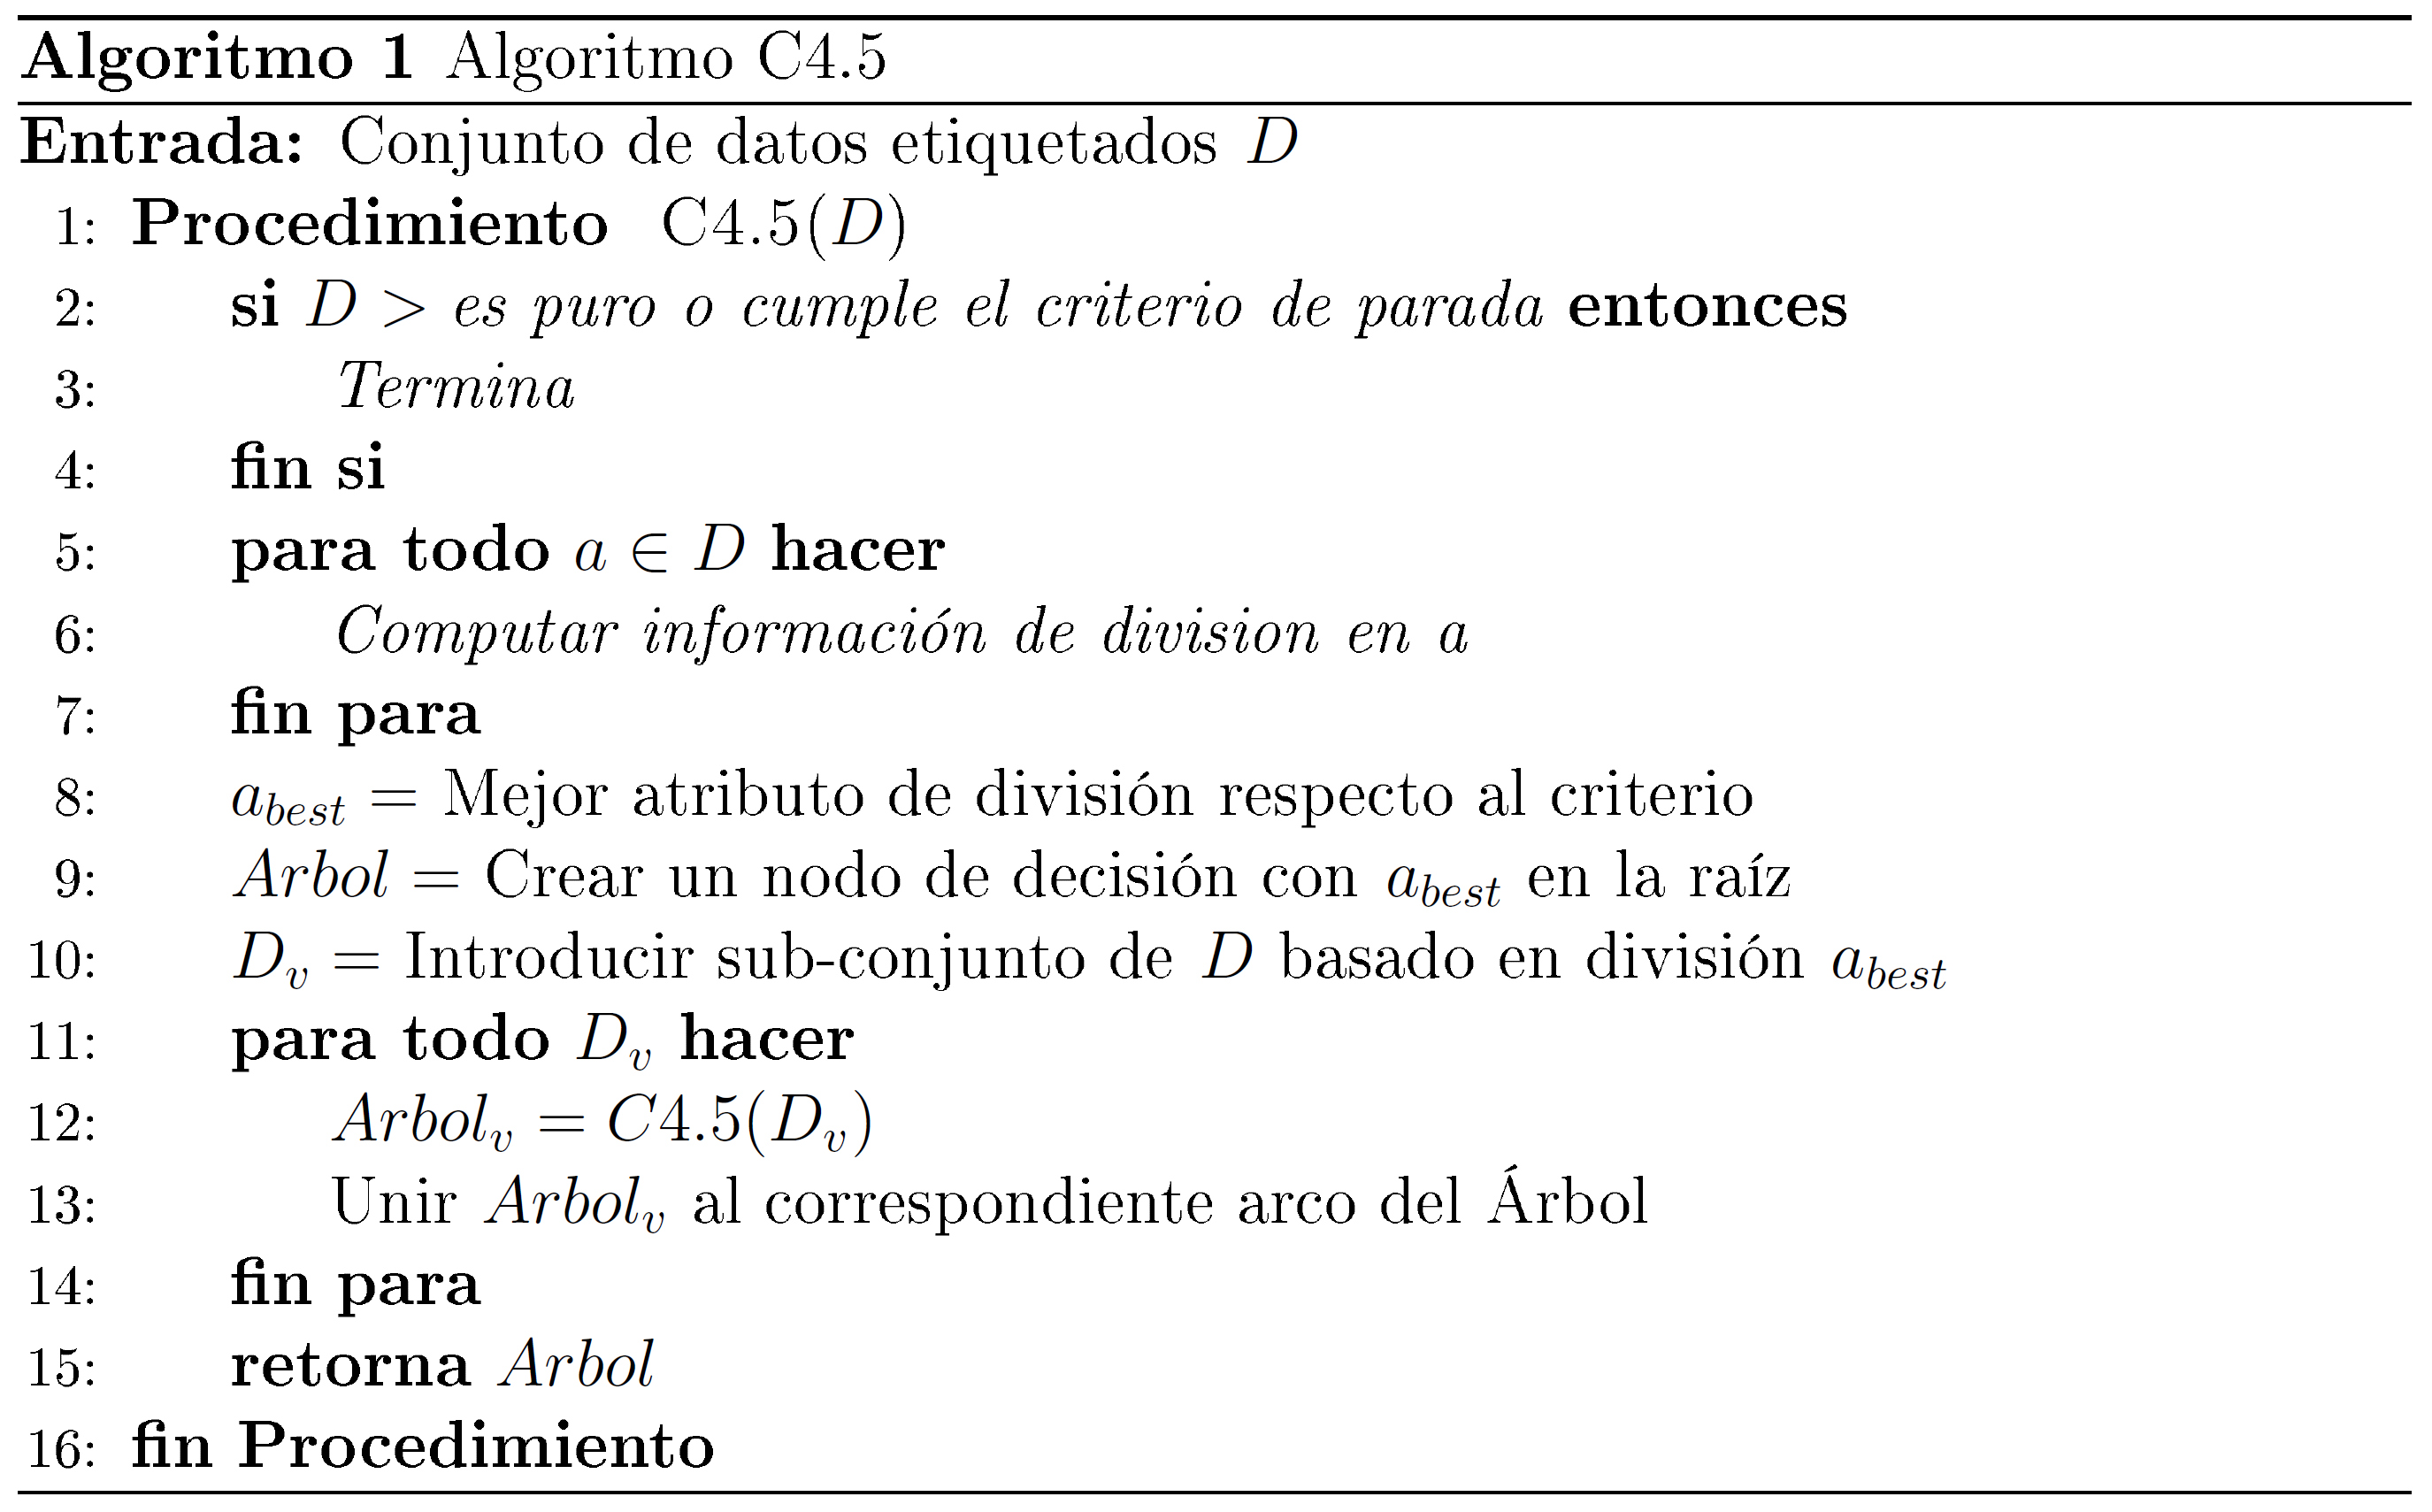
\includegraphics[width=\textheight]{propuesta/graphics/algoritmoC45}
	\par
\end{center}
\end{frame}
%
\begin{frame}[noframenumbering]
\frametitle{Anexo 1}
\framesubtitle{Selecci�n de atributo de divisi�n}

Podemos partir con esta tabla como datos iniciales de entrenamiento:

\setbeamercovered{transparent}
\begin{columns}

\column{0.3\textwidth}
	\pause{}
	\begin{itemize}
		\item Calcular Ganancia de cada atributo.		
		\item Calcular proporci�n de ganancia.
	\end{itemize}


\column{0.7\textwidth}
	\begin{center}
		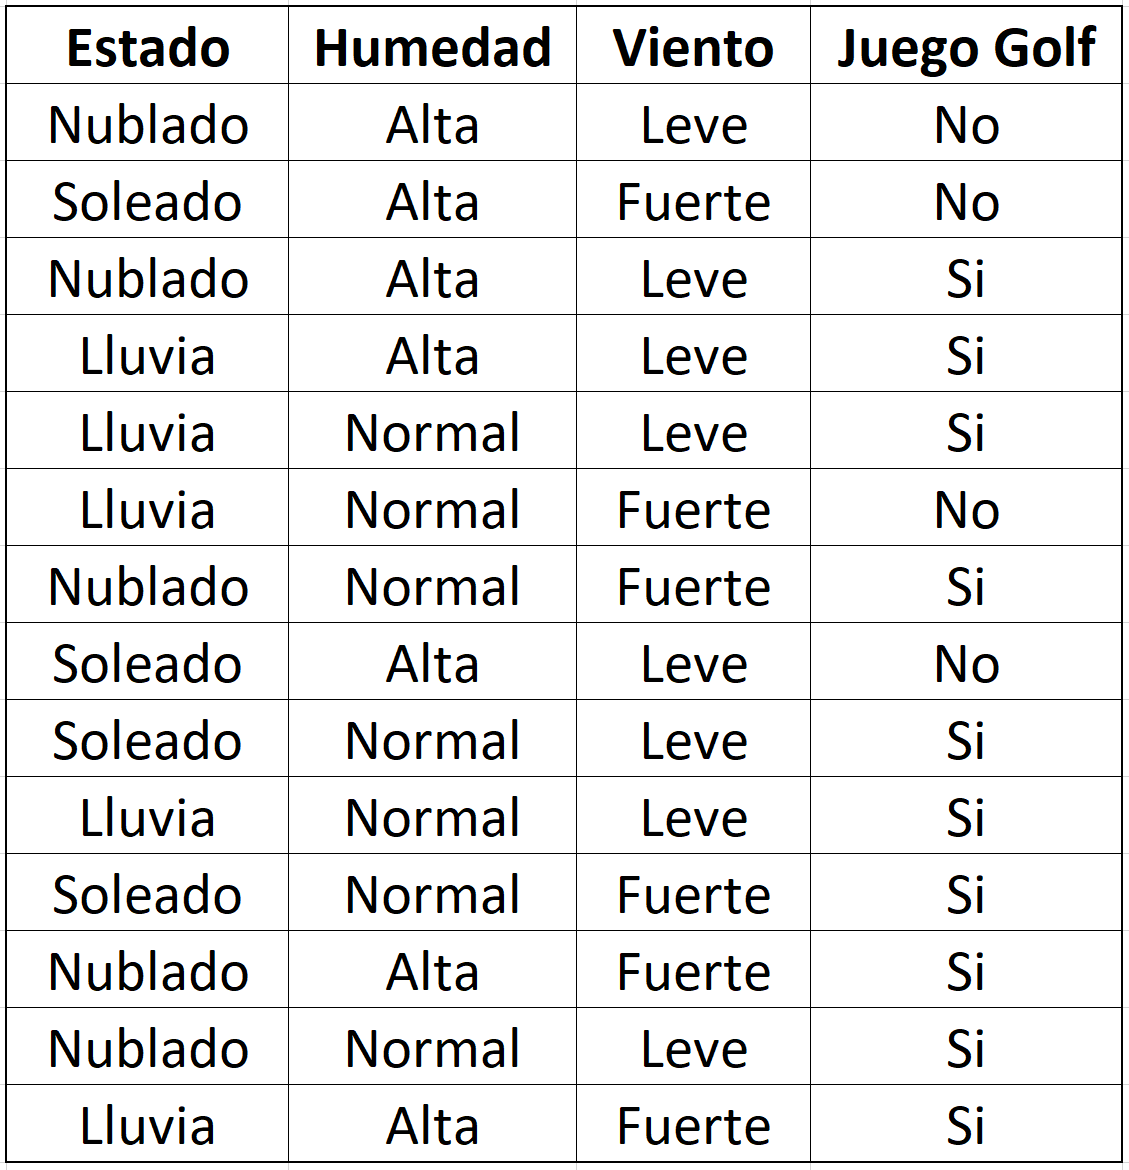
\includegraphics[width=0.7\textwidth]{anexo/graphics/tabla_inicial}
		\par
	\end{center}
\end{columns}
\end{frame}
%
\begin{frame}[noframenumbering]
\frametitle{Anexo 1}
\framesubtitle{Selecci�n de atributo de divisi�n}

Por ejemplo tomamos al atributo ESTADO:

\setbeamercovered{transparent}
\begin{columns}[t]
	
	\column{0.6\textwidth}
	\begin{center}
		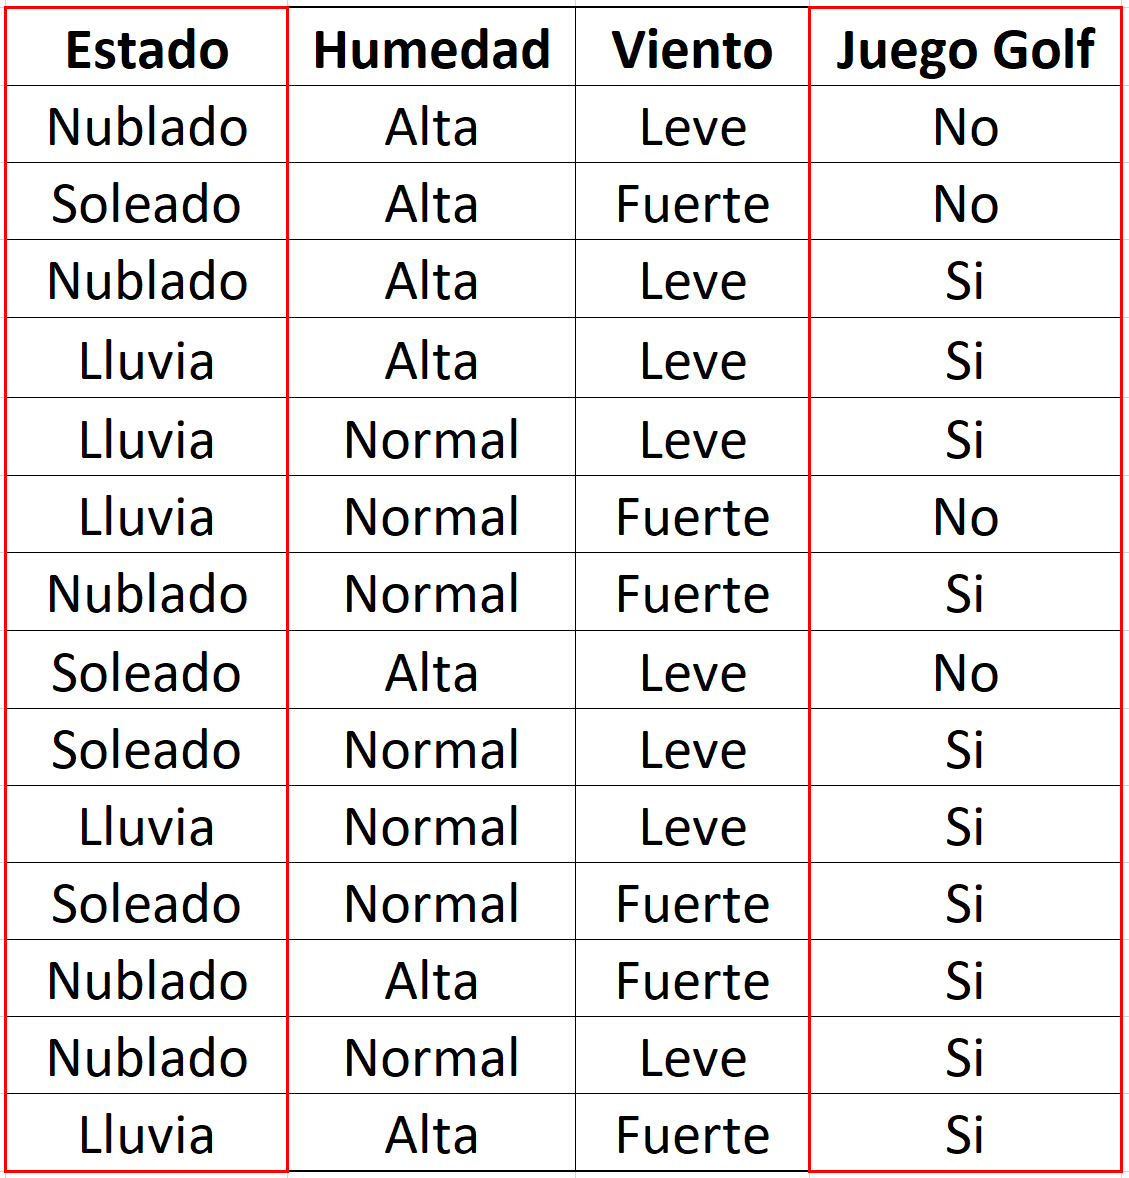
\includegraphics[width=0.7\textwidth]{anexo/graphics/tabla_estado}
		\par
	\end{center}
	
	
	\column{0.4\textwidth}
	\pause{}
	\begin{center}
		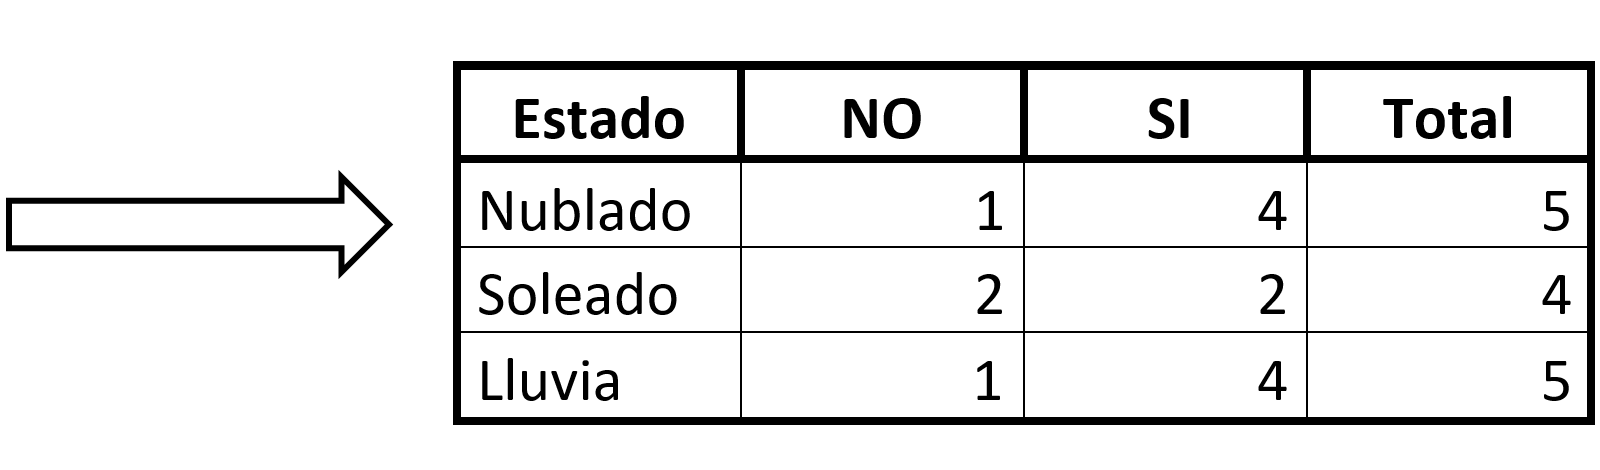
\includegraphics[width=1\columnwidth]{anexo/graphics/estado_resumen}
		\par
	\end{center}

	\scalebox{0.7}{%
		\vbox{
		\begin{equation*}Info(D) = - \displaystyle\sum_{i=1}^{m} p_{i}\log_2(p_{i}) \end{equation*}
		\begin{equation*}Info(D) = - \frac{4}{14}\log_2(\frac{4}{14}) - \frac{10}{14}\log_2(\frac{10}{14}) \end{equation*}
 		\begin{equation*}Info(D) = 0.863 \, bits \end{equation*}
	}}
\end{columns}
\end{frame}
%
\begin{frame}[noframenumbering]
\frametitle{Anexo 1}
\framesubtitle{Selecci�n de atributo de divisi�n}

Luego calculamos la ganancia al dividir en el atributo ESTADO:

\begin{equation*}
	\begin{split}
		Info_{Estado}(D) 	& = \frac{5}{14} \times ( -\frac{1}{5}\log_2(\frac{1}{5})-\frac{4}{5}\log_2(\frac{4}{5})  ) \\
							& + \frac{4}{14} \times ( -\frac{2}{4}\log_2(\frac{2}{4})-\frac{2}{4}\log_2(\frac{2}{4})  ) \\
							& + \frac{5}{14} \times ( -\frac{1}{5}\log_2(\frac{1}{5})-\frac{4}{5}\log_2(\frac{4}{5})  ) \\
							& = 0.801 \, bits.
	\end{split}
\end{equation*}

\begin{equation*}Gain(Estado) = Info(D) - Info_{Estado}(D) \end{equation*}
\begin{equation*}Gain(Estado) = 0.061 \, bits \end{equation*}

\end{frame}
%
\begin{frame}[noframenumbering,t]
\frametitle{Anexo 1}
\framesubtitle{Selecci�n de atributo de divisi�n}

Repitiendo los pasos para el resto de los atributos:

\begin{equation*}Gain(Humedad) = 0.012 \, bits \end{equation*}
\begin{equation*}Gain(Viento)  = 0.005 \, bits \end{equation*}
\begin{equation*}\alert<1>{Gain(Estado) = 0.061 \, bits}\end{equation*}

Por lo tanto el mejor atributo de divisi�n es \textit{ESTADO}

\end{frame}
%
\begin{frame}[noframenumbering]
\frametitle{Anexo 1}
\framesubtitle{Selecci�n de atributo de divisi�n}

Finalmente la divisi�n en el atributo ESTADO quedar�a de la siguiente manera:

\begin{overprint}

\onslide<1>
	\begin{center}
		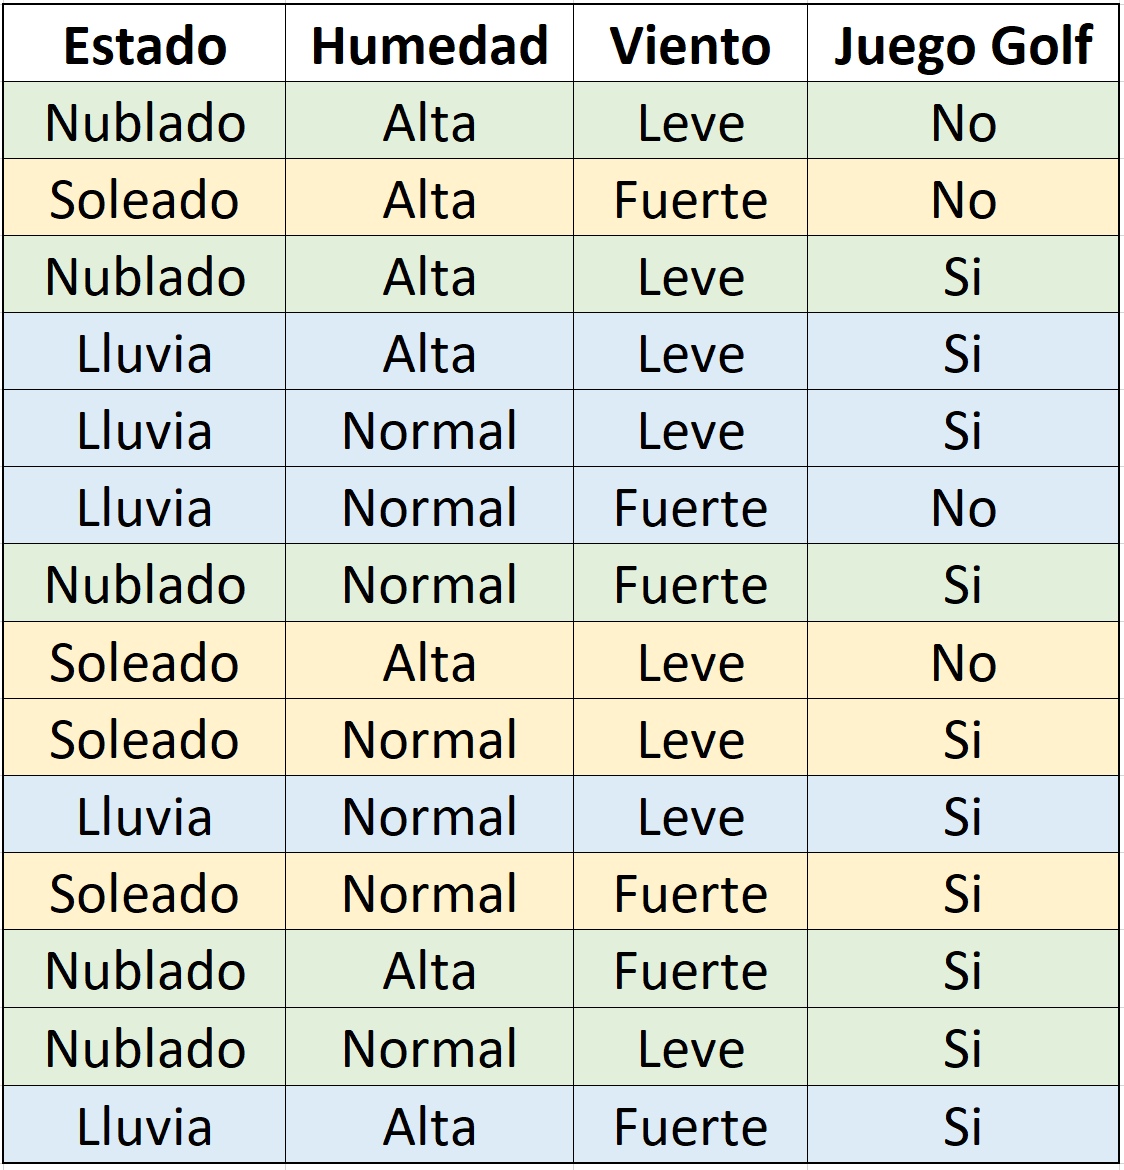
\includegraphics[width=0.5\textwidth]{anexo/graphics/tabla_coloreada}
		\par
	\end{center}

\onslide<2>
	\begin{center}
		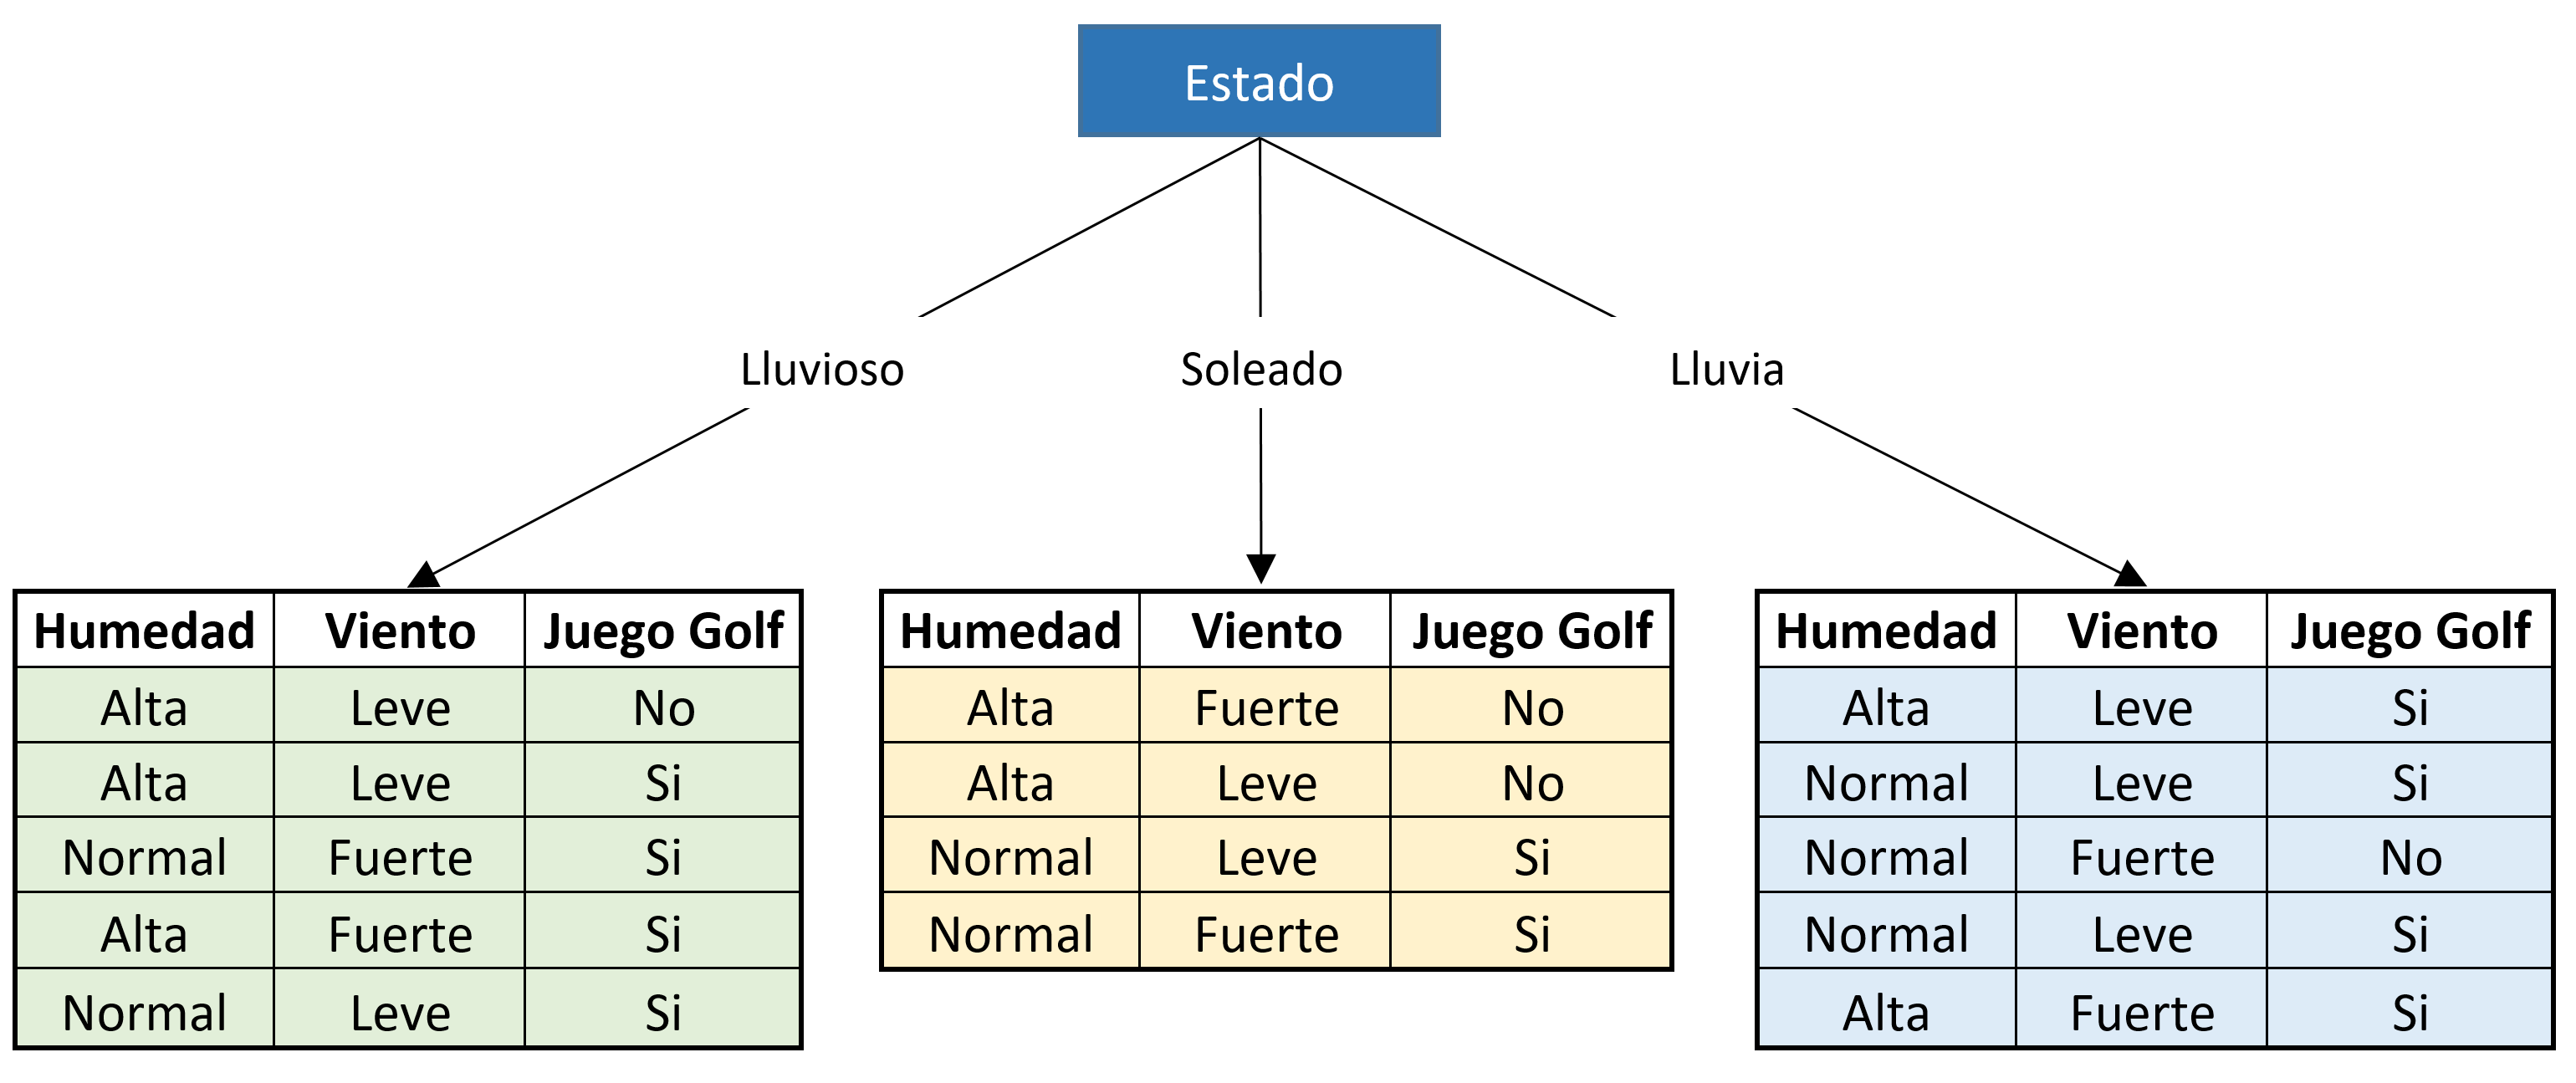
\includegraphics[width=0.9\textwidth]{anexo/graphics/primera_division}
		\par
	\end{center}

\end{overprint}

\end{frame}